\section{3D náhled}
3D náhled součástek LEGO je implementován s~využitím javascriptového frameworku Three.js. Tento framework disponuje velmi rozsáhlou a přehlednou dokumentací, včetně ukázek použití a je nejpoužívanějsím javascriptovým WebGL frameworkem \autocite{webgl-comparison}. Na základě těchto důvodů bylo rozhodnuto o~jeho využití v~tomto projektu.

% Three.js
% OrbitControls.js
% STLLoader.js

% \begin{listing}[htbp]
%         \begin{minted}{javascript}
%  $('#model-viewer').ModelViewer('{{ path('media_file', {'path':model.path}) }}');
%   \end{minted}
%   \caption{Inicializace 3D náhledu\label{modelviewer-initialization}}
% \end{listing}

% \begin{listing}[htbp]
%     \begin{minted}{javascript}
% ModelViewer.prototype.loadStl = function(model) {
%     var self = this;
%     var loader = new THREE.STLLoader();

%     loader.load(model,
%         function (geometry) {
%             self.addModel(geometry);
%         },
%         function(progress) {},
%         // Show error message
%         function(error) {
%             self.showError();
%         }
%     );
% };
%     \end{minted}
%     \caption{Načtení STL modelu pomocí Three.js\label{modelviewer-stl}}
% \end{listing}

Na obrázku \ref{obrazek-modelviewer} je možné vidět ukázku a možnosti implementovaného 3D náhledu.

\begin{figure}[htbp]
        \centering
        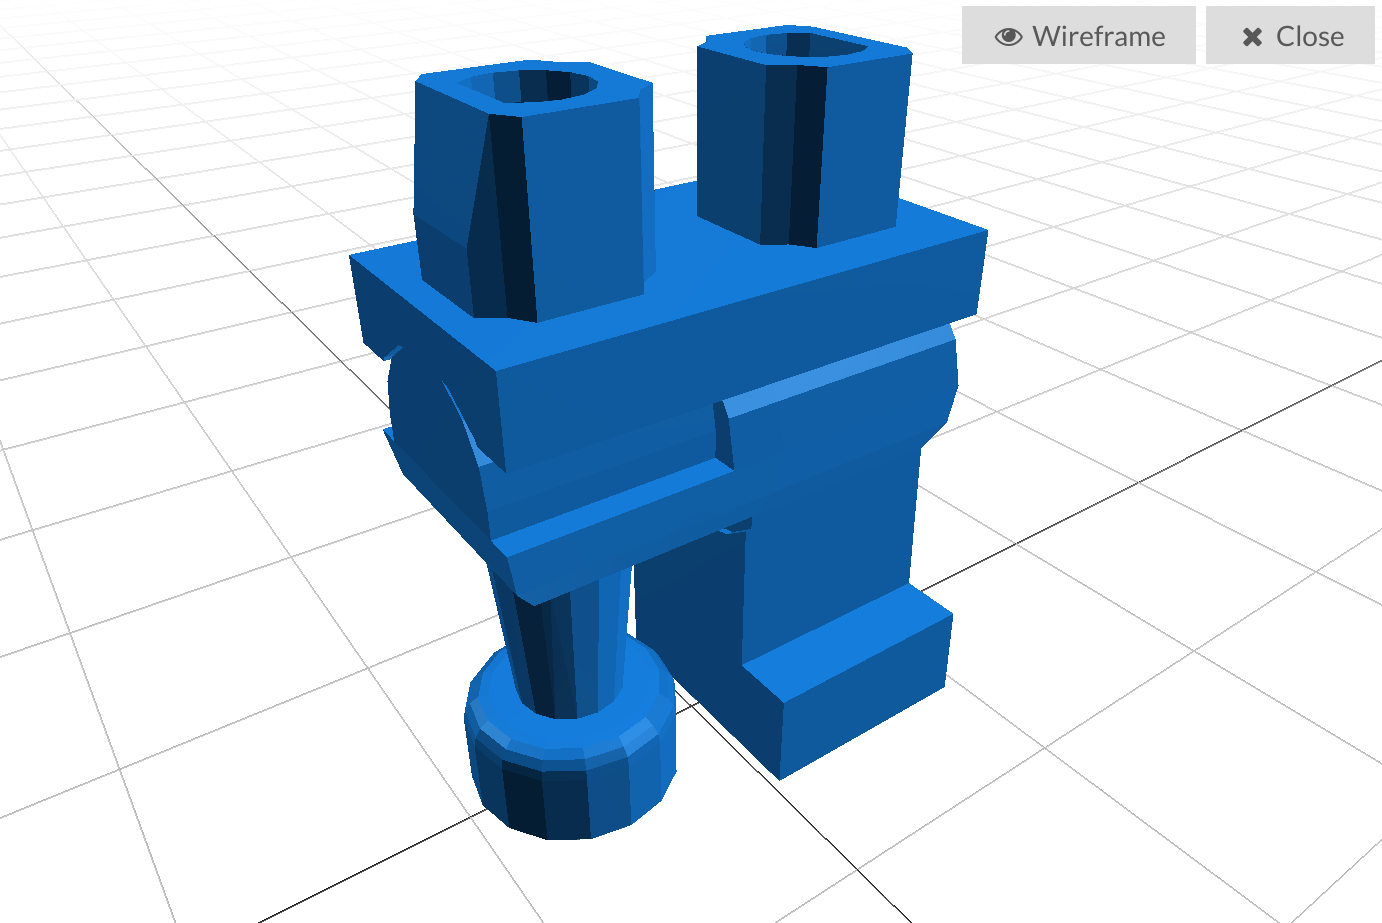
\includegraphics[width=0.48\textwidth,height=\textheight,keepaspectratio]{images/model-viewer-solid.png}
        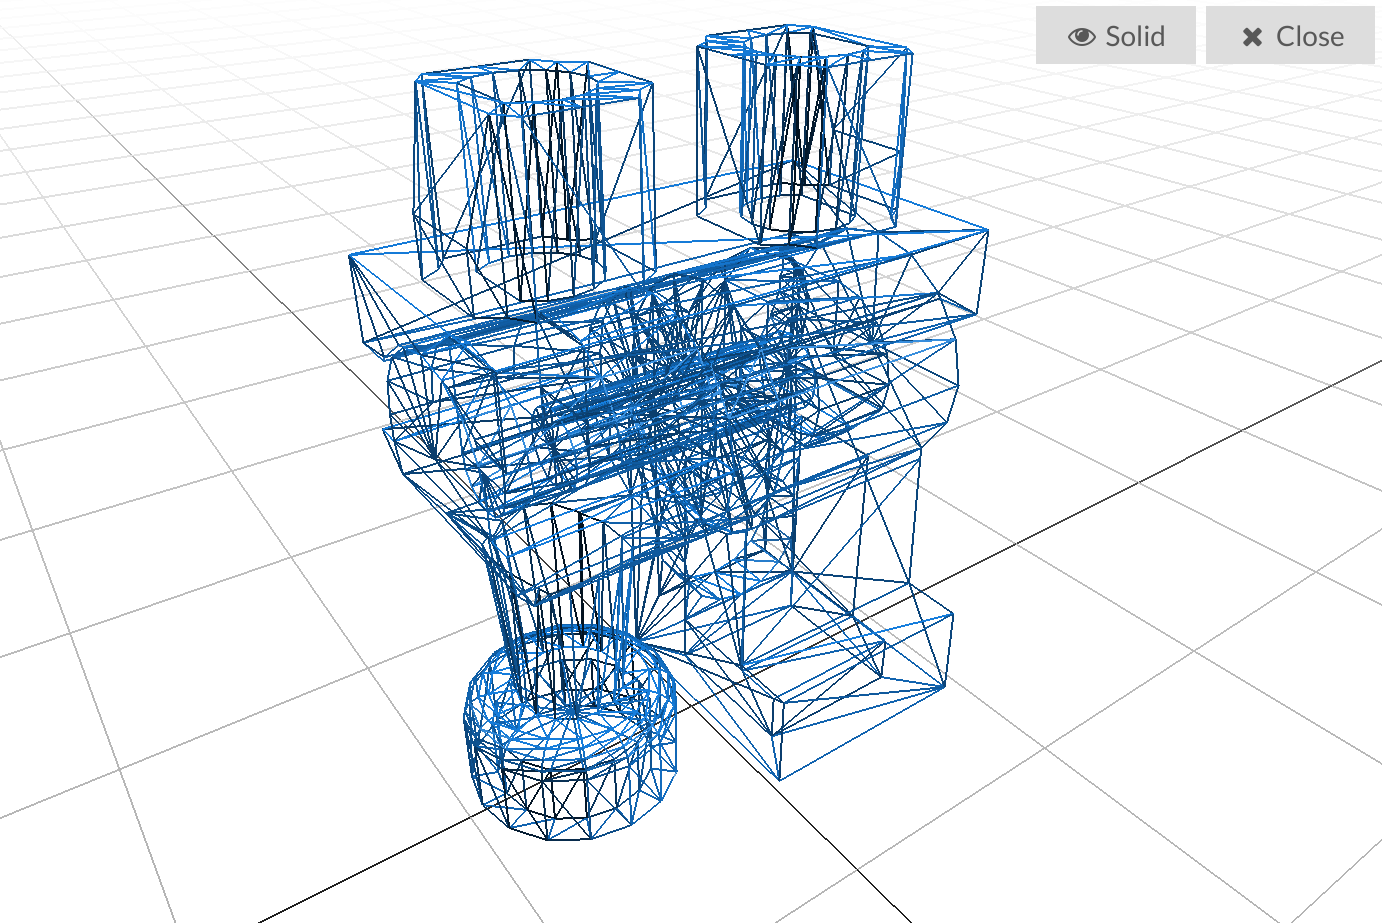
\includegraphics[width=0.48\textwidth,height=\textheight,keepaspectratio]{images/model-viewer-wireframe.png}
        \caption{3D náhled součástky \label{obrazek-modelviewer}}
\end{figure}